\documentclass[11pt]{article}

\hoffset        2mm 
\voffset        -15mm
\oddsidemargin  0mm
\topmargin      0.35in
\textwidth      6in
\textheight     9in

%\usepackage[parfill]{parskip}
\usepackage{graphicx}
\usepackage{amsmath}
%\usepackage{mathtools}
\usepackage{booktabs}
\usepackage{enumerate}
\usepackage{listings}
\usepackage{float}
\usepackage{epstopdf}

\begin{document}


\begin{center}
{\em \huge Higher-Order FEM Basis Functions on Triangular Prisms}\\[8mm]
{\LARGE By: Michael Hackemack}\\[3mm]
{\large July 9, 2016} \\[15mm]
\end{center}



%%%%%%%%%%%%%%%%%%%%%%%%%%%%%%%%%%%%%%%%%%%%%%%%%%%%%%%%%%%%%%%%%%%%%%
%%%%%%%%%%%%%%%%%%%%%%%%%%%%%%%%%%%%%%%%%%%%%%%%%%%%%%%%%%%%%%%%%%%%%%
\section{Introduction}
\label{sec::Introduction}

In this document, we derive higher-order basis functions

%%%%%%%%%%%%%%%%%%%%%%%%%%%%%%%%%%%%%%%%%%%%%%%%%%%%%%%%%%%%%%%%%%%%%%
%%%%%%%%%%%%%%%%%%%%%%%%%%%%%%%%%%%%%%%%%%%%%%%%%%%%%%%%%%%%%%%%%%%%%%
\section{Reference Basis Functions on a Triangle}
\label{sec::triref}

%%%%%%%%%%%%%%%%%%
%%%%%%%%%%%%%%%%%%
\subsection{Linear Basis Functions on the Reference Triangle}
\label{sec::triref_linear}

For this work, we choose the lagrange shape functions for triangles. The values and gradient equations for the linear basis functions on the reference triangle are given by

\begin{equation}
\label{eq::reftri_quad_basis_vals}
\begin{aligned}
b_1(x,y) \, =& \, (1-x-y) \\
b_2(x,y) \, =& \, x \\
b_3(x,y) \, =& \, y
\end{aligned}
\end{equation}

\noindent and

\begin{equation}
\label{eq::reftri_quad_basis_grads}
\begin{aligned}
\vec{\nabla}& b_1(x,y) \, = \, \left[ -1 , -1   \right] \\
\vec{\nabla}& b_2(x,y) \, = \, \left[ -1, 0   \right] \\
\vec{\nabla}& b_3(x,y) \, = \, \left[ 0, -1   \right] 
\end{aligned}
\end{equation}

\noindent respectively.

%%%%%%%%%%%%%%%%%%
%%%%%%%%%%%%%%%%%%
\subsection{Quadratic Basis Functions on the Reference Triangle}
\label{sec::triref_quadratic}


\begin{figure}[hbt]
\centering
	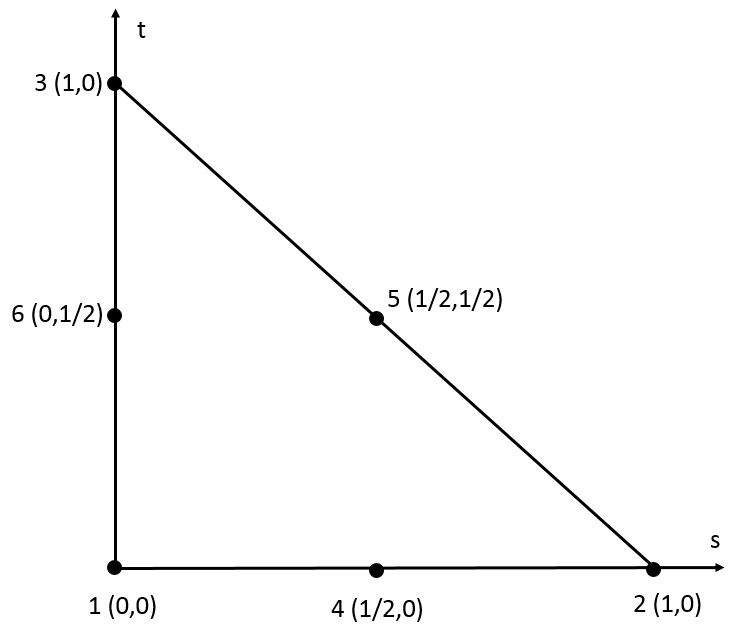
\includegraphics[width=3.0in]{./Figures/ref_triangle.jpg}
	\caption{Reference Triangle.}
\hspace{0.5cm}
\label{fig::ref_triangle}
\end{figure}

For this work, we choose the lagrange shape functions for triangles. The values and gradient equations for the quadratic basis functions on the reference triangle are given by

\begin{equation}
\label{eq::reftri_quad_basis_vals}
\begin{aligned}
b_1(x,y) \, =& \, (1-x-y) (1-2x-2y) \\
b_2(x,y) \, =& \, 2x(x-1/2) \\
b_3(x,y) \, =& \, 2y(y-1/2) \\
b_4(x,y) \, =& \, 4x (1-x-y) \\
b_5(x,y) \, =& \, 4xy\\
b_6(x,y) \, =& \, 4y (1-x-y)
\end{aligned}
\end{equation}

\noindent and

\begin{equation}
\label{eq::reftri_quad_basis_grads}
\begin{aligned}
\vec{\nabla}& b_1(x,y) \, = \, \left[ 4(x+y)-1 , 4(x+y)-1   \right] \\
\vec{\nabla}& b_2(x,y) \, = \, \left[ 4x-1, 0   \right] \\
\vec{\nabla}& b_3(x,y) \, = \, \left[ 0, 4y-1   \right] \\
\vec{\nabla}& b_4(x,y) \, = \, \left[ 4-8x, -4x   \right] \\
\vec{\nabla}& b_5(x,y) \, = \, \left[ 4y, 4x   \right] \\
\vec{\nabla}& b_6(x,y) \, = \, \left[ -4y, 4-8y   \right] 
\end{aligned}
\end{equation}

\noindent respectively.

%%%%%%%%%%%%%%%%%%
%%%%%%%%%%%%%%%%%%
\subsection{Cubic Basis Functions on the Reference Triangle}
\label{sec::triref_cubic}

For this work, we choose the lagrange shape functions for triangles. The values and gradient equations for the cubic basis functions on the reference triangle are given by

\begin{equation}
\label{eq::reftri_cubic_basis_vals}
\begin{aligned}
b_1(x,y) \, =& \, (1-x-y) (1/3-x-y) (2/3-x-y)\\
b_2(x,y) \, =& \, 2x(x-1/2) \\
b_3(x,y) \, =& \, 2y(y-1/2) \\
b_4(x,y) \, =& \, 4x (1-x-y) \\
b_5(x,y) \, =& \, 4xy\\
b_6(x,y) \, =& \, 4y (1-x-y) \\
b_7(x,y) \, =& \, 4y (1-x-y) \\
b_8(x,y) \, =& \, 4y (1-x-y) \\
b_9(x,y) \, =& \, 4y (1-x-y) \\
b_{10}(x,y) \, =& \, 4y (1-x-y) 
\end{aligned}
\end{equation}

%%%%%%%%%%%%%%%%%%
%%%%%%%%%%%%%%%%%%
\subsection{Quartic Basis Functions on the Reference Triangle}
\label{sec::triref_quartic}

For this work, we choose the lagrange shape functions for triangles.

%%%%%%%%%%%%%%%%%%%%%%%%%%%%%%%%%%%%%%%%%%%%%%%%%%%%%%%%%%%%%%%%%%%%%%
%%%%%%%%%%%%%%%%%%%%%%%%%%%%%%%%%%%%%%%%%%%%%%%%%%%%%%%%%%%%%%%%%%%%%%
\section{Reference Basis Functions on a Triangular Prism}
\label{sec::triprismref}

%%%%%%%%%%%%%%%%%%%%%%%%%%%%%%%%%%%%%%%%%%%%%%%%%%%%%%%%%%%%%%%%%%%%%%
%%%%%%%%%%%%%%%%%%%%%%%%%%%%%%%%%%%%%%%%%%%%%%%%%%%%%%%%%%%%%%%%%%%%%%
\section{Computing the Jacobian Transformation}
\label{sec::jacobian}


%%%%%%%%%%%%%%%%%%%%%%%%%%%%%%%%%%%%%%%%%%%%%%%%%%%%%%%%%%%%%%%%%%%%%%
%%%%%%%%%%%%%%%%%%%%%%%%%%%%%%%%%%%%%%%%%%%%%%%%%%%%%%%%%%%%%%%%%%%%%%
\section{Conclusions}
\label{sec::conclusions}

%%%%%%%%%%%%%%%%%%%%%%%%%%%%%%%%%%%%%%%%%%%%%%%%%%%%%%%%%%%%%%%%%%%%%%
%%%%%%%%%%%%%%%%%%%%%%%%%%%%%%%%%%%%%%%%%%%%%%%%%%%%%%%%%%%%%%%%%%%%%%
\bibliographystyle{ans}
\bibliography{references}


\end{document}


